\documentclass{beamer}
\usepackage{tikz}
\usetikzlibrary{shapes.geometric, arrows.meta}

\tikzset{
    block/.style = {rectangle, rounded corners, minimum width=3cm, minimum height=1cm,text centered, draw=black, fill=red!30},
    line/.style = {draw, -Latex},
    cloud/.style = {draw, ellipse,fill=red!20, node distance=3cm,
                    minimum height=2em}
}

\begin{document}

\begin{frame}{¿Qué es Musixtex?}
    \begin{itemize}
        \item Es posible incrustar un gráfico de mapa de bits dentro de un gráfico vectorial, pero no es posible incrustar información vectorial en un mapa de bits.
        \item Las imágenes en los monitores de las computadoras también son mapas de bits, al igual que las salidas de impresoras, escáneres y dispositivos similares.
    \end{itemize}
    
    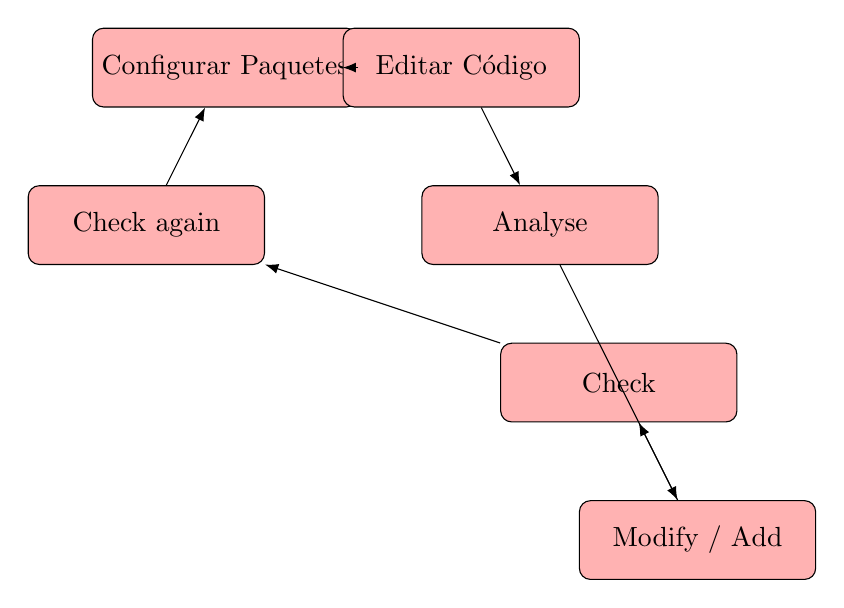
\begin{tikzpicture}[node distance = 2cm, auto]
        \node [block] (configurar) {Configurar Paquetes};
        \node [block, below of=configurar, xshift=-1cm] (check) {Check again};
        \node [block, right of=configurar, xshift=1cm] (editar) {Editar Código};
        \node [block, below of=editar, xshift=1cm] (analise) {Analyse};
        \node [block, below of=analise, xshift=1cm] (check2) {Check};
        \node [block, below of=check2, xshift=1cm] (modify) {Modify / Add};
        
        \path [line] (configurar) -- (editar);
        \path [line] (editar) -- (analise);
        \path [line] (analise) -- (modify);
        \path [line] (modify) -- (check2);
        \path [line] (check2) -- (check);
        \path [line] (check) -- (configurar);
    \end{tikzpicture}
\end{frame}

\end{document}